\section{Ziel des Versuches}
Wenn zwei schwingende Systeme so miteinander verbunden sind, dass diese aufeinander einwirken können, werden diese als gekoppelt bezeichnet. Von besonderem Interesse ist der Energieübergang, zwischen den gekoppelten Systemen. In diesem Versuch wird der gekoppelte Schwingkreis untersucht. Dafür werden die Resonanzeffekte und die Fundamentalschwingungen beobachtet.

\section{Theoretische Grundlage}
\label{sec:Theorie}
Für diesen Versuch wird ein Schwingkreis verwendet, da sich bei diesem die Frequenzen und Amplituden besser bestimmen lassen, als bei zwei Fadenpendeln welche über eine Feder gekoppelt sind.

\subsection{Verhalten kapazitiv gekoppelte Schwingkreise}
Im folgenden werden zwei gleiche Schwingkreise, welche durch die Kapazität  $C_\text{K}$ gekoppelt sind, untersucht(siehe Abbildung \ref{fig:GekSch}).

\begin{figure}[H] %gekoppelter Schwingkreis
	\centering
	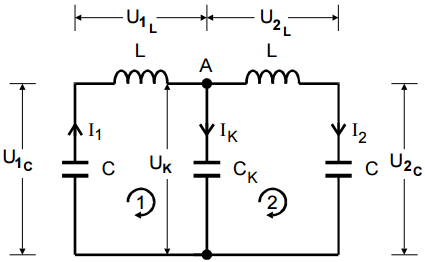
\includegraphics[height=6cm]{picture/GekoppelterSchwingkreis.PNG}
	\caption{Schaltung eines kapazitiv gekoppeltem Schwingkreises \cite{sample}.}
	\label{fig:GekSch}
\end{figure}

Der Schwingkreis liegt den Kirchhoffschen Regeln zu Grunde. Die erste der beiden Regeln besagt, dass die Summe der eingehenden und ausgehende Ströme an einem Knoten gleich Null ist.
\begin{equation}
  \text{Knotenregel} : \sum_{\text{k=1}}^\text{n} I_\text{k} = 0
  \label{eqn:K1}
\end{equation}
Die zweite Regel besagt, dass sich bei einer Geschlossenen Masche alle Teilspannungen, bei einem Umlauf zu Null addieren.
\begin{equation}
  \text{Maschenregel} : \sum_{\text{k=1}}^\text{n} U_\text{k} = 0 \ .
  \label{eqn:K2}
\end{equation}
Damit ergibt sich für beide Maschen
\begin{equation}
	U_\text{C} + U_\text{L} + U_\text{K} = 0 \ ,
\end{equation}
wobei für die Spannung in der Spule
\begin{equation*}
	U_\text{L} = L \dot{I}
\end{equation*}
gilt und für die Kondensatorspannung gilt
\begin{equation*}
	U_\text{C} = \frac{1}{C} \int \! \! \! \! I dt \ .
\end{equation*}
Außerdem ergibt sich für den Strom am Knotenpunkt A
\begin{equation*}
	I_1 = I_\text{K} + I_2 \ .
\end{equation*}
Mit diesen Beziehungen ergeben sich für beide Maschen mit anschließender Differentiation nach t folgende Differentialgleichungen
\begin{equation}
	L \ddot{I}_1 + \frac{1}{C} I_1 + \frac{1}{C_\text{K}}(I_1 - I_2) = 0
	\label{eqn:Masche1}
\end{equation}
und
\begin{equation}
	L \ddot{I}_2 + \frac{1}{C} I_2 + \frac{1}{C_\text{K}}(I_1 - I_2) = 0 \ .
	\label{eqn:Masche2}
\end{equation}
Um die beiden Differentialgleichungssysteme zu lösen werden neue Variablen eingeführt und zwar Summe und Differenz der Einzelströme. Damit ergeben sich aus 	\ref{eqn:Masche1} und \ref{eqn:Masche2}
\begin{equation}
	L \frac{d^2}{d t^2}(I_1 + I_2) + \frac{1}{C}(I_1 + I_2) = 0
	\label{eqn:DGL1}
\end{equation}
und
\begin{equation}
	L \frac{d^2}{d t^2}(I_1 - I_2) + \left(\frac{1}{C} + \frac{2}{C_\text{K}} \right)(I_1 - I_2) = 0 \ .
	\label{eqn:DGL2}
\end{equation}
Die Lösung von \ref{eqn:DGL1} ist
\begin{equation}
	(I_1 + I_2)(t) = (I_{1_0} + I_{2_0}) \cos \left(\frac{t}{\sqrt{LC}} \right) \ ,
\end{equation}
mit der Schwingungsfrequenz
\begin{equation}
	\nu^+ = \frac{1}{2 \pi \sqrt{LC}} \ .
	\label{eqn:vp}
\end{equation}
Die Lösung von \ref{eqn:DGL2} ist
\begin{equation}
	(I_1 - I_2)(t) = (I_{1_0} - I_{2_0}) \cos \left(\frac{t}{\sqrt{L \left(\frac{1}{C} + \frac{2}{C_\text{K}} \right)^{-1}}} \right) \ ,
\end{equation}
mit der Schwingungsfrequenz
\begin{equation}
\nu^- = \frac{1}{2 \pi \sqrt{L \left(\frac{1}{C} + \frac{2}{C_\text{K}} \right)^{-1}}} \ .
	\label{eqn:vm}
\end{equation}
Für die ursprünglichen Variablen $I_1$ und $I_2$ ergibt sich nun
\begin{equation}
	I_1(t) = \frac{1}{2}(I_{1_0} + I_{2_0}) \cos(2 \pi \nu^+ t) + \frac{1}{2}(I_{1_0} - I_{2_0}) \cos(2 \pi \nu^- t)
	\label{eqn:I1}
\end{equation}
und
\begin{equation}
	I_2(t) = \frac{1}{2}(I_{1_0} + I_{2_0}) \cos(2 \pi \nu^+ t) - \frac{1}{2}(I_{1_0} - I_{2_0}) \cos(2 \pi \nu^- t) \ .
	\label{eqn:I2}
\end{equation}
An dieser Stelle werden nun zwei Spezialfälle des gekoppelten Systems betrachtet. \\
\textbf{erster Spezialfall:} \ ($I_{1_0} = I_{2_0}$) \\
Wenn zu Beginn des Versuches die Schwingkreise gleich stark und in Phase ausgelenkt werden, fällt in den Gleichungen \ref{eqn:I1} und \ref{eqn:I2} jeweils die Differenzschwingung raus. Das heißt beide Systeme schwingen mit der Frequenz $\nu^+$ und es liegt zu keinem Zeitpunkt eine Spannung an dem Koppelkondensator an. \\
\textbf{zweiter Spezialfall:} \ ($I_{1_0} = -I_{2_0}$) \\
Wenn zu Beginn des Versuches die Schwingkreise gleichstark und mit entgegengesetzter Phase ausgelenkt werden, fällt in den Gleichungen \ref{eqn:I1} und \ref{eqn:I2} jeweils die Summenschwingung raus. Das heißt beide Systeme schwingen mit der Frequenz $\nu^-$ und es liegt die maximale Spannung an dem Koppelkondensator an. \\
Die beiden Speziallfälle werden auch als Fundamentalschwingungen des gekoppelten Systems bezeichnet.\\
\\
Wird hingegen nur einer der Schwingkreise ausgelenkt ($I_{2_0} = 0$ oder $I_{1_0} = 0$) folgt:
\begin{equation}
	I_1(t) = I_{1_0} \cos(\pi (\nu^+ + \nu^-)t) \cos(\pi (\nu^+ - \nu^-)t)
\end{equation}
\begin{equation}
	I_2(t) = I_{2_0} \sin(\pi (\nu^+ + \nu^-)t) \sin(\pi (\nu^+ - \nu^-)t) \ .
\end{equation}
In der folgenden Abbildung wird der Verlauf der Ströme $I_1(t)$ und $I_2(t)$ dargestellt.

\begin{figure}[H]
	\centering
	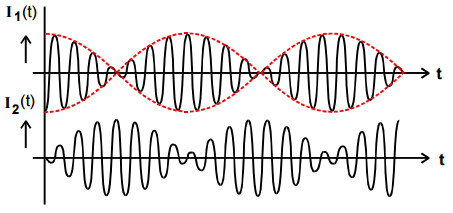
\includegraphics[height=5cm]{picture/Schwebungsfrequenz.PNG}
	\caption{Zeitabhängigkeit der Ströme in den Schwingkreisen im Falle einer Schwebung \cite{sample}.}
	\label{fig:SchFre}
\end{figure}

Die Amplitude des Schwingung ändert sich mit der Schwebungsfrequnez $\nu^- - \nu^+$, während das System mit der Frequenz
\begin{equation*}
	\frac{\nu^+ + \nu^-}{2} \approx \nu^+
\end{equation*}
schwingt.

\subsection{Abhängigkeit des Stromes von der Frequenz}
Wenn einer der Schwingkreise von einer angelegten Sinusspannung angeregt wird(siehe Abb. \ref{fig:AngSch}),
\begin{figure}[H]
	\centering
	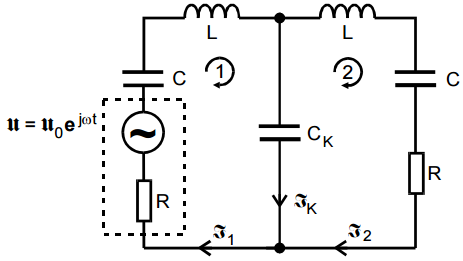
\includegraphics[height=5cm]{picture/AngeregterSchwingkreis.PNG}
	\caption{Gekoppelte Schwingkreise mit eingebautem Sinusgenerator \cite{sample}.}
	\label{fig:AngSch}
\end{figure}
so ergibt sich über die Kirchhoffsche Maschenregel zu
\begin{equation}
	\text{Kreis 1:} \ U = (z_\text{C} + z_\text{L} + z_{\text{C}_\text{K}} + z_\text{R})I_1 - z_{\text{C}_\text{K}}I_2
\end{equation}
und
\begin{equation}
	\text{Kreis 2:} \ 0 = (z_\text{C} + z_\text{L} + z_{\text{C}_\text{K}} + z_\text{R})I_2 - z_{\text{C}_\text{K}}I_1 \ .
\end{equation}
Für die einzelnen Impedanzen gilt
\begin{align*}
	z_\text{C} & = \frac{1}{i \omega C} \ , \\
	z_\text{L} & = i \omega L \ \ \text{und} \\
	z_\text{R} & = R \ .
\end{align*}
Nach Elimination von $I_1$ folgt für $I_2$
\begin{equation}
	I_2 = U \frac{\frac{-i}{\omega C_\text{K}}} {\left(i \omega L - i \left(\frac{1}{\omega C} + \frac{1}{\omega C_\text{K}} \right) + R \right)^2 + \frac{1}{\omega^2 C^2_\text{K}}} \ .
\end{equation}
Nach Trennung in Real- und Imaginärteil erhält man für $|I_2|$ mit der Abkürzung
\begin{align*}
	Z(\omega) := \omega L - \frac{1}{\omega C} - \frac{1}{\omega C_\text{K}}
\end{align*}
\begin{equation}
		|I_2| = |U| \frac{1}{\sqrt{4 \omega^2 C^2_\text{K} R^2 Z(\omega)^2 + \left(\frac{1}{\omega C_\text{K}} - \omega C_\text{K} Z(\omega)^2 + \omega R^2 C_\text{K} \right)^2}} := |U| \cdot |\pmb{\varrho}|
		\label{eqn:BetragI}
\end{equation}
An der Gleichung \ref{eqn:BetragI} wird deutlich, dass $|I_2|$ für $\omega \to 0$ und für $\omega \to \infty$ gegen null geht und bei den Frequenzen $\omega^+$ und $\omega^-$ seine Maxima besitzt.
\begin{equation}
	|\pmb{\varrho}(\omega^+)| = \frac{1}{R \sqrt{4 + \frac{R^2 C^2_\text{K}}{LC}}}
\end{equation}
\begin{equation}
	|\pmb{\varrho}(\omega^-)| = \frac{1}{R \sqrt{4 + \frac{R^2 C^2_\text{K}}{LC} \left(1 + \frac{C}{C_\text{K}} \right)}}
\end{equation}
Im folgenden wird $|\pmb{\varrho}(\omega^{+/-})|$ zu $\frac{1}{2R}$ genähert.

\subsection{Fehlerrechnung}
Sämtliche Fehlerrechnungen werden mit Hilfe von Python 3.4.3 durchgeführt.
\subsubsection{Mittelwert}
Der Mittelwert einer Messreihe $x_\text{1}, ... ,x_\text{n}$ lässt sich durch die Formel
\begin{equation}
	\overline{x} = \frac{1}{N} \sum_{\text{k}=1}^\text{N} x_k
	\label{eqn:ave}
\end{equation}
berechnen. Die Standardabweichung des Mittelwertes beträgt
\begin{equation}
	\Delta \overline{x} = \sqrt{ \frac{1}{N(N-1)} \sum_{\text{k}=1}^\text{N} (x_\text{k} - \overline{x})^2}
	\label{eqn:std}
\end{equation}

\subsubsection{Gauß'sche Fehlerfortpflanzung}
Wenn $x_\text{1}, ..., x_\text{n}$ fehlerbehaftete Messgrößen im weiteren Verlauf benutzt werden, wird der neue Fehler $\Delta f$ mit Hilfe der Gaußschen Fehlerfortpflanzung angegeben.
\begin{equation}
	\Delta f = \sqrt{\sum_{\text{k}=1}^\text{N} \left( \frac{ \partial f}{\partial x_\text{k}} \right) ^2 \cdot (\Delta x_\text{k})^2}
	\label{eqn:var}
\end{equation}

\subsubsection{Lineare Regression}
Die Steigung und y-Achsenabschnitt einer Ausgleichsgeraden werden gegebenfalls mittels Linearen Regression berechnet.
\begin{equation}
	y = m \cdot x + b
	\label{eqn:reg}
\end{equation}
\begin{equation}
	m = \frac{ \overline{xy} - \overline{x} \overline{y} } {\overline{x^2} - \overline{x}^2}
	\label{eqn:reg_m}
\end{equation}
\begin{equation}
	b = \frac{ \overline{x^2}\overline{y} - \overline{x} \, \overline{xy}} { \overline{x^2} - \overline{x}^2}
	\label{eqn:reg_b}
\end{equation}
